\chapter{Desenvolvimento \label{chap:Desenvolvimento}}

% Resumo opcional. Comentar se não usar.
% \resumodocapitulo{Resumo opcional.}


\section{Biblioteca} \label{sec:lib}

O servidor da partida apresenta, como já mencionado, um protocolo de comunicação e sintaxe de mensagens específica. Uma biblioteca de interfaceamento foi desenvolvida com o objetivo de abstrair os detalhes de comunicação de construção de mensagens e facilitar, assim, o desenvolvimento dos programas jogadores. Esta abordagem já é comum na categoria e existem soluções de código aberto como a \textit{librcsc}, utilizada por várias equipes, usualmente atreladas ao agente base \textit{agent2d}, desenvolvidas pela equipe \textit{HELIOS}.

A biblioteca própria foi desenvolvida em linguagem Go como forma de modernização e diversificação da base de código utilizada pelas equipes. A biblioteca cobre uma parte considerável das possibilidades previstas no protocolo de comunicação e foi programada de modo a ser facilmente expansível de acordo com o lançamento de novas versões do servidor.

\subsection{Arquitetura do código}
A biblioteca possui três pacotes internos: \textit{playerclient}, \textit{trainerclient} e \textit{rcsscommon}. Os dois primeiros dizem respeito aos dois tipos de programas que podem se conectar ao servidor da partida: jogadores e treinadores. O terceiro engloba todas as funcionalidades utilizadas por ambos clientes, além de informações gerais sobre parâmetros da partida, como coordenadas de bandeiras do campo e modos de jogo.

Os dois clientes desenvolvidos possuem as funcionalidades necessárias para se conectar ao servidor, ouvir mensagens via protocolo UDP, decodificá-las e então executar uma ação em forma de mensagem codificada e enviada ao servidor.

\subsection{Decodificação de Codificação de Mensagens}
\label{sec:messsages}
% lexer -> analisador léxico
% parser -> analisador sintático
A decodificação de mensagens, por sua vez, foi feita em duas camadas: um analisador léxico e um analisador sintático. O lexer passa pelas mensagens em formato string e retira todas as informações que ela contém. O analisador sintático estrutura essas informações em estruturas de dados para que possam ser utilizadas fora da biblioteca. As informações recebidas e decodificadas são, em sua maioria, dados dos sensores do jogador.
\begin{center}



\begin{tabular}{c}
\begin{lstlisting}
(see 37 ((f c b) 16.6 -1 -0 -0.8))
\end{lstlisting}
\end{tabular}

Exemplo de mensagem codificada.


\begin{tabular}{c}
\begin{lstlisting}
SightSymbols{
	Time: 37,
	ObjMap: map[string][]string{
		"f c b":    {"16.6", "-1", "-0", "-0.8"},
	},
}
\end{lstlisting}
\end{tabular}

Mensagem após passar pelo analisador léxico.



\begin{tabular}{c}
\begin{lstlisting}
SightData{
	Time: 37,
	Ball: nil,
	Lines: LineArray{},
	Flags: FlagArray{
		{
			ID:        rcsscommon.FlagCenterBot,
			Distance:  16.6,
			Direction: -1,
		},
	},
}
\end{lstlisting}
\end{tabular}

Mensagem após passar pelo analisador sintático.

\end{center}

\section{Definição dos Estados}
\par As informações de estado são fornecidas pelos sensores do jogador. Há três sensores presentes que entregam informações, em forma de mensagens, para o agente: sensor auditivo, sensor visual e sensor corporal.
\par Além de ser necessário tratar as mensagens recebidas, como demonstrado na seção \ref{sec:messsages}, é necessário tratar alguns dos estados para dar mais informações ao agente. 

\subsection{Sensores}
\par Os sensores são responsáveis por todas as informações que o jogador tem do ambiente. Eles são modelados de forma a emular características de sensores reais, então, dessa forma, um sensor pode ``perder'' informações caso a variável medida esteja longe, como será evidenciado no modelo do sensor visual.
\subsubsection{Sensor Auditivo}

As mensagens do sensor auditivo são do seguinte formato:

\textit{(hear Tempo Remetente "mensagem")}

Onde \textit{Tempo} é o número do ciclo em que a mensagem foi ouvida e \textit{Remetente} é descrição de quem enviou a mensagem. O \textit{Remetente} pode ser o árbitro, outros jogadores, um dos treinadores ou o próprio jogador.

No escopo deste trabalho, apenas as mensagens do árbitro serão consideradas, não sendo implementada nenhuma forma de comunicação direta entre os jogadores.

\subsubsection{Sensor Visual}
\label{sec:visual}
As mensagens do sensor visual contém as posições relativas referentes a cada objeto dentro do campo de visão do jogador. Esses objetos podem ser outros jogadores, marcadores como bandeiras e linhas (Figura \ref{fig:flags}) e a bola. O formato genérico é este:

\textit{(see (Objeto1)(Objeto2)(Objeto3)...(ObjetoN))}

Onde cada objeto tem o seguinte formato:

\textit{((NomeDoObjeto) Distância Direção VariaçãoDeDistância VariaçãoDeDireção DireçãoDoCorpo DireçãoDaCabeça)}

Sendo a distância e a direção dados em coordenadas polares, assim como suas variações. As informações de direção do corpo e da cabeça só aparecem quando o objeto em questão é um outro jogador.

\begin{figure}[H]
	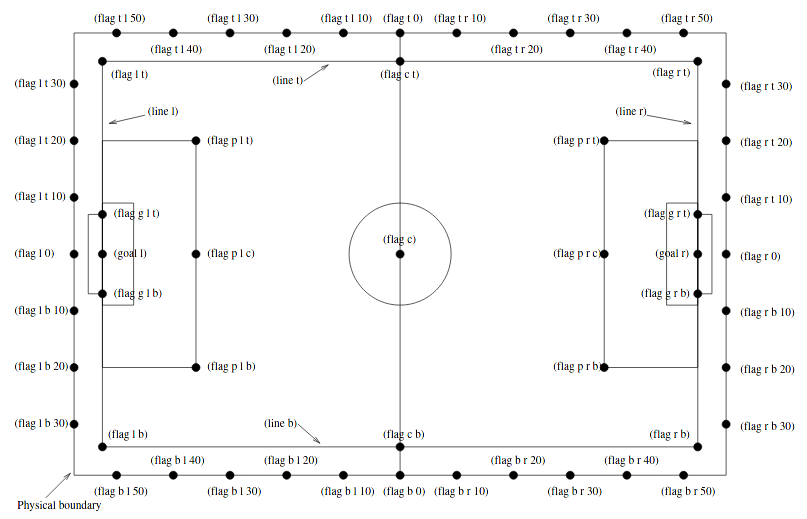
\includegraphics[width=0.9\linewidth]{figs/flags.png}
	\centering
	\caption{Indicadores espalhados pelo campo para que o agente possa estimar sua posição absoluta \cite{rcssmanual2003}.}
	\label{fig:flags}
\end{figure}

A riqueza de detalhes a respeito das informações obtidas depende da distância entre o objeto e o jogador. Por exemplo, caso esteja sendo visto outro jogador a uma distância muito grande, talvez seja impossível determinar o número de sua camisa ou até mesmo a qual time ele pertence. Em contrapartida, para jogadores próximos, é fornecido até mesmo a direção para a qual ele está olhando.

\subsubsection{Sensor Corporal}

O sensor corporal contém informações sobre o estado físico do jogador. Entre elas sua energia, que é consumida a cada ação tomada como chute ou arrancada (Seção \ref{sec:actions}), sua própria velocidade e direção de movimento, a direção de sua cabeça e a quantidade de cartões de advertência recebidos.

\subsection{Estimação e Tratamento de Estados}
\par Os sensores do jogador fornecem somente informações em coordenadas polares relativas ao próprio jogador. Desta forma, ele possui informações de distância e direção para a bola, demais jogadores, bandeiras do campo e linhas do campo. 
\par Com esses dados, entretanto, é possível estimar as coordenadas cartesianas absolutas no campo de todas as entidades de interesse. As bandeiras do campo são fixas e possuem coordenadas conhecidas, seção \ref{sec:visual}. Portanto, a transformação da informação polar e relativa para uma cartesiana e absoluta da posição do próprio jogador é direta utilizando trigonometria básica. 
\par A partir da informação de posição absoluta do próprio jogador e de sua direção é possível calcular as posições para o resto das entidades.
% TODO: decidir se falar do NotSeenBallFor é ok já que a gente não treinou com ele
\par É possível, também, extrair estados úteis a partir das informações dos sensores, como por exemplo um estado que representa a quanto tempo o jogador não vê a bola. Este estado pode ser determinante para que o jogador escolha buscar a bola.

\subsection{Discretização}
% TODO
\section{Definição de Ações}
% TODO: mover detalhamento de ações para cá

\subsection{Discretização do Espaço de Ações}

\subsection{Definição de Comportamentos}

\section{Seleção de Comportamentos e Ações}

\section{Ambiente de Treinamento}

O ambiente de treinamento consiste em uma base de código que importa a biblioteca detalhada na seção \ref{sec:lib}. Um formato geral foi definido e desenvolvido a fim de tornar os experimentos fáceis de adaptar, bastando mudar alguns trechos do código.

\subsection{Laço de Treinamento}

De forma geral o laço de treinamento obedece o pseudo-código apresentado.

\begin{tabular}{c}
	\begin{lstlisting}
		definir parametros
		inicializar pesos de treinamento
		enquanto o estado nao e terminal:
			conectar jogador
			laco para cada passo da partida:
				escolher acao de acordo com a politica e o estado
				observar novo estado e recompensa
				treinar pesos
				estado <- novo estado
	\end{lstlisting}
\end{tabular}

O laço interno é onde efetivamente os algoritmos de treinamento são implementados, portanto este trecho é alterado a depender da técnica de aprendizagem por reforço utilizada.


\subsection{Experimentos}

% listar experimentos que serão apresentados a seguir
% double q tabular
% double q tabular behaviors